\chapter{Managing Linux Based Firewalls}
	
\section{Understanding Firewalld Operation}
\textbf{Firewalld} provides primarily two interfaces to manage it: \verb|firewall-cmd|, a command line utility to manage its functions, and \verb|firewall-config| a graphical user interface to do the same. However, since most servers don't provide a GUI or even have a window manager installed, this second options isn't always available.

\verb|firewall-cmd| has a list of pre-defined zones and services that can be accessed with \verb|--get-<parameter>| options. To list the parameter that are actually active at the moment, we use \verb|--list-parameter| option instead. For exmaple, we use \verb|--list-services| to get the list of currently active services:

\vspace{-15pt}
\begin{minted}{console}
# firewall-cmd --get-zones
block dmz drop external home internal public trusted work
# firewall-cmd --get-services
RH-Satellite-6 amanda-client amanda-k5-client bacula bacula-client bitcoin bitcoin-rpc bitcoin-testnet bitcoin-testnet-rpc ceph ceph-mon cfengine condor-collector ctdb dhcp dhcpv6 dhcpv6-client dns docker-registry dropbox-lansync elasticsearch freeipa-ldap freeipa-ldaps freeipa-replication freeipa-trust ftp ganglia-client ganglia-master high-availability http https imap imaps ipp ipp-client ipsec iscsi-target kadmin kerberos kibana klogin kpasswd kshell ldap ldaps libvirt libvirt-tls managesieve mdns mosh mountd ms-wbt mssql mysql nfs nrpe ntp openvpn ovirt-imageio ovirt-storageconsole ovirt-vmconsole pmcd pmproxy pmwebapi pmwebapis pop3 pop3s postgresql privoxy proxy-dhcp ptp pulseaudio puppetmaster quassel radius rpc-bind rsh rsyncd samba samba-client sane sip sips smtp smtp-submission smtps snmp snmptrap spideroak-lansync squid ssh synergy syslog syslog-tls telnet tftp tftp-client tinc tor-socks transmission-client vdsm vnc-server wbem-https xmpp-bosh xmpp-client xmpp-local xmpp-server
# firewall-cmd --list-services 
ssh dhcpv6-client
\end{minted}
\vspace{-10pt}	

\noindent
These predefined services are stored in the folder \verb|/usr/lib/firewalld/services| as \textit{XML} files, listing the service name and the associated ports and protocol:

\vspace{-15pt}
\begin{minted}{xml}
<?xml version="1.0" encoding="utf-8"?>
<service>
	<short>LDAP</short>
	<description>Lightweight Directory Access Protocol (LDAP) server</description>
	<port protocol="tcp" port="389"/>
</service>

\end{minted}
\vspace{-10pt}	

\noindent
For certain services, certian kernel modules may also be loaded, such as in the case of \textit{FTP}, for which the \verb|/usr/lib/firewalld/services/ftp.xml| has:

\vspace{-15pt}
\begin{minted}{xml}
<service>
	<short>FTP</short>
	<description>FTP is a protocol used for remote file transfer. If you plan to make your FTP server publicly available, enable this option. You need the vsftpd package installed for this option to be useful.</description>
	<port protocol="tcp" port="21"/>
	<module name="nf_conntrack_ftp"/>
</service>
\end{minted}
\vspace{-10pt}	

\noindent
The kernel module \verb|nf_conntrack_ftp| is loaded for the service by firewalld. The services in the \verb|/usr/lib/firewalld/services| folder are system defined and any changes made to them are overwritten with every system update. So, the user defined services go in the folder \verb|/etc/firewalld/services| with the added advantage of overwriting the settings of the system defined services in \verb|/usr/lib/firewalld/services|. 

Every change made using firewall-cmd is not permanent, unless explicitly made permanent using the \verb|--permanent| option. Even then, the firewall has to be reloaded using the \verb|--reload| option for the changes to take effect. Finally, the state of the firewall can be guaged with:

\vspace{-15pt}
\begin{minted}{console}
# firewall-cmd --state
running
\end{minted}
\vspace{-10pt}	

\noindent
The firewalld configurations are stored in \verb|/etc/firewalld/firewalld.conf|:

\vspace{-15pt}
\begin{minted}{bash}
# firewalld config file

# default zone
# The default zone used if an empty zone string is used.
# Default: public
DefaultZone=public

# Minimal mark
# Marks up to this minimum are free for use for example in the direct 
# interface. If more free marks are needed, increase the minimum
# Default: 100
MinimalMark=100

# Clean up on exit
# If set to no or false the firewall configuration will not get cleaned up
# on exit or stop of firewalld
# Default: yes
CleanupOnExit=yes

# Lockdown
# If set to enabled, firewall changes with the D-Bus interface will be limited
# to applications that are listed in the lockdown whitelist.
# The lockdown whitelist file is lockdown-whitelist.xml
# Default: no
Lockdown=no

# IPv6_rpfilter
# Performs a reverse path filter test on a packet for IPv6. If a reply to the
# packet would be sent via the same interface that the packet arrived on, the 
# packet will match and be accepted, otherwise dropped.
# The rp_filter for IPv4 is controlled using sysctl.
# Default: yes
IPv6_rpfilter=yes

# IndividualCalls
# Do not use combined -restore calls, but individual calls. This increases the
# time that is needed to apply changes and to start the daemon, but is good for
# debugging.
# Default: no
IndividualCalls=no

# LogDenied
# Add logging rules right before reject and drop rules in the INPUT, FORWARD
# and OUTPUT chains for the default rules and also final reject and drop rules
# in zones. Possible values are: all, unicast, broadcast, multicast and off.
# Default: off
LogDenied=off

# AutomaticHelpers
# For the secure use of iptables and connection tracking helpers it is
# recommended to turn AutomaticHelpers off. But this might have side effects on
# other services using the netfilter helpers as the sysctl setting in
# /proc/sys/net/netfilter/nf_conntrack_helper will be changed.
# With the system setting, the default value set in the kernel or with sysctl
# will be used. Possible values are: yes, no and system.
# Default: system
AutomaticHelpers=system
\end{minted}
\vspace{-10pt}	

\noindent
The value of the default zone can be directly obtained with:

\vspace{-15pt}
\begin{minted}{console}
# firewall-cmd --get-default-zone 
public
\end{minted}

	\section{Configuring Firewalld Services and Zones}
The very first thing to remember while working with \textbf{firewalld} is to stop and disable the \textbf{iptables} service, which used to be the old firewalling solution and is still available as a service in certain versions of RHEL 7, but is incompatible with firewalld. For this, we use:

\vspace{-15pt}
\begin{minted}{console}
# systemctl disable iptables
# systemctl stop iptables
# systemctl mask iptables
\end{minted}
\vspace{-10pt}	

\noindent
The very last command is masking of a service, which is creating a link to \verb|/dev/null| from the service unit file in \verb|/etc/systemd/system/iptables.service|, so that it may never even accidentally be started. Any service masked in this manner can be reactivated using \verb|systemctl unmask <serviceName>|. 

Firewalld can have multiple active zones. An overview of all the active zones can be obtained by:

\vspace{-15pt}
\begin{minted}{console}
# firewall-cmd --get-active-zones 
public
interfaces: ens33 ens37 br0 team0
\end{minted}
\vspace{-10pt}	

\noindent
This is particularly useful in cases of configurations of private subnets on one zone, assigned to an interface and the internet on another zone, assigned to another interface. 

Every single configuration detail for the default zone can be obtained with the command:

\vspace{-15pt}
\begin{minted}{console}
# firewall-cmd --list-all
public (active)
  target: default
  icmp-block-inversion: no
  interfaces: ens33 ens37 br0 team0
  sources: 
  services: ssh dhcpv6-client
  ports: 
  protocols: 
  masquerade: no
  forward-ports: 
  source-ports: 
  icmp-blocks: 
  rich rules: 
\end{minted}
\vspace{-10pt}	

\noindent
The config details for another, specific zone can be obtained by filtering with:

\vspace{-15pt}
\begin{minted}{console}
# firewall-cmd --list-all --zone=dmz 
dmz
  target: default
  icmp-block-inversion: no
  interfaces: 
  sources: 
  services: ssh
  ports: 
  protocols: 
  masquerade: no
  forward-ports: 
  source-ports: 
  icmp-blocks: 
  rich rules: 
\end{minted}
\vspace{-10pt}	

\subsection{Adding and removing services}
To add a service to a particular zone, the \verb|--zone=<zoneName>| option has to be used. Without it, the currently active zone will have the service added to it. The command to add the \verb|ftp| service for example, is:

\vspace{-15pt}
\begin{minted}{console}
# firewall-cmd --list-services 
ssh dhcpv6-client
# firewall-cmd --add-service=ftp 
success
# firewall-cmd --list-services 
ssh dhcpv6-client ftp
# firewall-cmd --reload 
success
# firewall-cmd --list-services 
ssh dhcpv6-client
# firewall-cmd --add-service=ftp --permanent 
success
# firewall-cmd --list-services 
ssh dhcpv6-client
# firewall-cmd --reload 
success
# firewall-cmd --list-services 
ssh dhcpv6-client ftp
\end{minted}
\vspace{-10pt}	

\noindent
At first we only add the service to runtime by excluding the \verb|--permanent| tag. Then upon reload of the firewall, the service disappears. When the service is made permanent, the changes are written to a configuration file, and not the runtime, and thus the firewall needs to be reloaded for the changes to take effect. The removal of a service also takes this form, and can be done by the command:

\vspace{-15pt}
\begin{minted}{console}
# firewall-cmd --remove-service=ftp --permanent 
success
# firewall-cmd --reload 
success
# firewall-cmd --list-services 
ssh dhcpv6-client
\end{minted}
\vspace{-10pt}	

\subsection{Letting an IP address through}
To only allow traffic from a particular IP (or a subnet) via the firewall, we use the command:

\vspace{-15pt}
\begin{minted}{console}
# firewall-cmd --permanent --add-source=10.0.0.0/24 
success
# firewall-cmd --reload
success
# firewall-cmd --list-all
public (active)
  target: default
  icmp-block-inversion: no
  interfaces: ens33 ens37 br0 team0
  sources: 10.0.0.0/24
  services: ssh dhcpv6-client
  ports: 
  protocols: 
  masquerade: no
  forward-ports: 
  source-ports: 
  icmp-blocks: 
  rich rules: 
\end{minted}
\vspace{-10pt}	

\subsection{Unblocking a specific port}
In the case of unblocking a port, we need to specify the protocol associated with the port as well, in the format \verb|<port#>/<protocol>|. Thus, the command to unblock the port 53 (DNS) becomes:

\vspace{-15pt}
\begin{minted}{console}
# firewall-cmd --permanent --add-port=53/tcp
success
# firewall-cmd --reload
success
# firewall-cmd --list-all
public (active)
  target: default
  icmp-block-inversion: no
  interfaces: ens33 ens37 br0 team0
  sources: 10.0.0.0/24
  services: ssh dhcpv6-client
  ports: 53/tcp
  protocols: 
  masquerade: no
  forward-ports: 
  source-ports: 
  icmp-blocks: 
  rich rules: 
\end{minted}

\section{Creating Services Files}
To create our own service file for firewalld, we need to copy an existing service file into the \verb|/etc/firewalld/services/| directory, to prevent errors stemming from creating the service file from scratch. So, to create a service file we do:

\vspace{-15pt}
\begin{minted}{console}
# cp /usr/lib/firewalld/services/ldap.xml /etc/firewalld/services/custom.xml
\end{minted}
\vspace{-10pt}	

\noindent
Now, if our application requires the port 8888 unblocked for the TCP protocol, we edit the file's contents to:

\vspace{-15pt}
\begin{minted}{xml}
<?xml version="1.0" encoding="utf-8"?>
<service>
	<short>Custom</short>
	<description>Service for custom application</description>
	<port protocol="tcp" port="8888"/>
</service>
\end{minted}
\vspace{-10pt}	

\noindent
Now, if we were to use the \verb|--get-services| option, we wouldn't see our custom service till we reloaded the firewall:

\vspace{-15pt}
\begin{minted}{console}
# firewall-cmd --get-services | grep -Eo " c(\S)*"
ceph
ceph-mon
cfengine
condor-collector
ctdb
# firewall-cmd --reload
success
# firewall-cmd --get-services | grep -Eo " c(\S)*"
ceph
ceph-mon
cfengine
condor-collector
ctdb
custom
\end{minted}
\vspace{-10pt}	

\noindent
The \verb|grep -E| enables extended RegEx while the \verb|-o| flag only prints the matching part. The expression \verb|c(\S)*| prints anything starting with a c till a whitespace character is encountered. Using a service file can be advantageous because we can add/remove multiple ports and protocols simultaneously from the firewall configuration using just a single command. 

	\section{Configuring Rich Firewall Rules}
There are two types of firewall rules: \textit{direct rules} and \textbf{rich rules}. Direct rules are hand-coded rules inserted by administrators that are processed before anything else in the zones. However, it isn't recommended to use them since they're a last resort when rules cannot be added via rich rules. 

Rich rules are used to create custom rules via an expressive language that can accomplish tasks that basic syntax can't, thus allowing us to create complex rules in an easy to understand manner. The documentation for this \textit{rich language} can be found using \verb|man 5 firewalld.richlanguage|. To work with rich rules, we must understand the order in which firewalld handles rules. The order is:

\begin{enumerate}
	\item Port Forward and Masquerading rules.
	\item Login rules
	\item Allow rules
	\item Deny rules
\end{enumerate}

\noindent
Thus any packet that the firewall encounters is first checked against the port forwarding and masquerading rules, then the login rules, then the allow rules and finally the deny rules. Note that there are no longer \textit{chains} as found while using \textbf{iptables}. To manage rich rules, the \verb|firewall-cmd| command has 4 subcommands:

\begin{itemize}
	\item \verb|--add-rich-rule=<rule>|
	\item \verb|--remove-rich-rule=<rule>|
	\item \verb|--query-rich-rule=<rule>|
	\item \verb|--list-rich-rules|
\end{itemize}

\subsection{Basic Syntax for Rich Rules}
The basic syntax of the rich language is:

\vspace{-15pt}
\begin{minted}{bash}
rule [family="ipv4|ipv6"]
  [source [not] address="address[/mask]"|mac="mac-address"|ipset="ipset"]
  [destination [not] address="address[/mask]"]
  service|port|protocol|icmp-block|icmp-type|masquerade|forward-port|source-port
  [log [prefix="prefix text"] [level="log level"] [limit value="rate/duration"]]
  [audit [limit value="rate/duration"]]
  [accept|reject|drop|mark] [limit value="rate/duration"]
\end{minted}
\vspace{-10pt}	

\noindent
Each of the criteria can have the values:

\noindent
\begin{tabular}{rM{0.48}M{0.3}}
	\toprule
	\textbf{Terms} &\textbf{Usage} &\textbf{Example}\\
	\midrule
	\textbf{service}	&service name="service name" &\verb|service name="ftp"|\\
	\midrule
	\textbf{port}	&port port="portid[-portid]" &\verb|port port="53"| \verb|protocol="udp"| \textbf{OR}\\
	&protocol="tcp|udp" &\verb|port port="8100-8115"|\\
	\midrule
	\textbf{protocol}	&protocol value="protocol value" &\verb|protocol value="cbt"|\\
	\midrule
	\textbf{icmp-block}	&icmp-block name="icmptype name" &\verb|icmp-block| \verb|name="echo-reply"|\\
	\midrule
\end{tabular}

\noindent
\begin{tabular}{rM{0.48}M{0.3}}
	\midrule
	\textbf{masquerade}	&masquerade &\verb|masquerade|\\
	\midrule
	\textbf{icmp-type}	&icmp-type name="icmptype name" &\verb|icmp-type name="des-| \verb|tination-unreachable"|\\
	\midrule
	\textbf{forward port}	&forward-port port="port value" protocol="tcp|udp" &\verb|forward-port port="69"| \verb|protocol="tcp"|\\
	&to-port="port value" to-addr="address" &\verb|to-port="1058"| \verb|to-addr="10.0.0.69"|\\
	\midrule
	\textbf{source port}	&source-port port="port value" protocol="tcp|udp" &\verb|source-port port="2022"| \verb|protocol="tcp"|\\
	\bottomrule
\end{tabular}

\noindent
For both icmp-block and icmp-type, the argument is of type \textit{icmptype} which can be listed using: \verb|firewall-cmd --get-icmptypes|. The log and audit options are a way to include logging. Also, it is only possible to limit the log/audit functionality or the action itself. 

\subsubsection{Actions}
\vspace{-10pt}
There are three types of actions that we need to be concerned with for any packet that meets the criteria set in the firewall: \textbf{accept}, \textbf{reject} or \textbf{drop}. With \textit{accept}, all matching packets will be accepted. With \textit{reject}, all matching packets will be rejected and the source will receive an ICMP error message (default ICMPv6). In the case of \textit{drop}, the packets are rejected silently, and the source gets no error messages. 

\subsection{Creating Rich Rules}
\subsubsection{Allowing/Denying packets from an IP address}
\vspace{-10pt}
The rich rule to deny all traffic from \verb|10.0.0.100| will be:

\vspace{-15pt}
\begin{minted}{console}
# firewall-cmd --permanent --zone=public --add-rich-rule='rule family=ipv4 source address=10.0.0.100/32 reject'
success
# firewall-cmd --reload
success
# firewall-cmd --list-rich-rules 
rule family="ipv4" source address="10.0.0.100/32" reject
\end{minted}
\vspace{-10pt}	

\subsubsection{Allowing/Denying a service based on Rate Limitation}
\vspace{-10pt}
To limit the number of http packets flowing through the firewall that are allowed into the network up to 3 per minute, we use:

\vspace{-15pt}
\begin{minted}{console}
# firewall-cmd --permanent --add-rich-rule='rule service name=http limit value=3/m accept'
success
# firewall-cmd --reload 
success
# firewall-cmd --list-rich-rules 
rule family="ipv4" source address="10.0.0.100/32" reject
rule service name="http" accept limit value="3/m"
\end{minted}
\vspace{-10pt}	

\subsubsection{Allowing/Denying a Protocol}
\vspace{-10pt}
There are several protocols listed in the \verb|/etc/protocols|	file, from which the firewall can look up a particular protocol being used. The file describes several protocols from the TCP/IP subsystem in the format: \verb|<protocol name> <number> <alias> <comments>| The first few lines of \verb|/etc/protocols| are: 

\vspace{-15pt}
\begin{minted}{bash}
ip      0       IP              # internet protocol, pseudo protocol number
hopopt  0       HOPOPT          # hop-by-hop options for ipv6
icmp    1       ICMP            # internet control message protocol
igmp    2       IGMP            # internet group management protocol
ggp     3       GGP             # gateway-gateway protocol
ipv4    4       IPv4            # IPv4 encapsulation
st      5       ST              # ST datagram mode
tcp     6       TCP             # transmission control protocol
cbt     7       CBT             # CBT, Tony Ballardie <A.Ballardie@cs.ucl.ac.uk>
egp     8       EGP             # exterior gateway protocol
...
\end{minted}
\vspace{-10pt}	

\noindent
Now, if we want all packets using the \textit{CBT} protocol to pass through the firewall, we use the command:

\vspace{-15pt}
\begin{minted}{console}
# firewall-cmd --permanent --add-rich-rule='rule protocol value=cbt accept'
success
# firewall-cmd --reload
success
# firewall-cmd --list-rich-rules 
rule family="ipv4" source address="10.0.0.100/32" reject
rule service name="http" accept limit value="3/m"
rule protocol value="cbt" accept
\end{minted}
\vspace{-10pt}	

\subsubsection{More complicated rules}	
A rule to allow TCP requests from the network 10.0.0.0/24 from ports 7900-7905 will be:

\vspace{-15pt}
\begin{minted}{console}
# firewall-cmd --permanent --add-rich-rule='rule family=ipv4 source address="10.0.0.0/24" port port="7900-7905" protocol=tcp accept'
success
# firewall-cmd --reload
success
# firewall-cmd --list-rich-rules 
rule family="ipv4" source address="10.0.0.100/32" reject
rule service name="http" accept limit value="3/m"
rule protocol value="cbt" accept
rule family="ipv4" source address="10.0.0.0/24" port port="7900-7905" protocol="tcp" accept
\end{minted}
\vspace{-10pt}	

\subsubsection{Logging}
\vspace{-10pt}
The rule to log SSH packets passing through the firewall at a limit of 2 per min in the syslog with a prefix of "ssh", a level of "notice":

\vspace{-15pt}
\begin{minted}{console}
# firewall-cmd --permanent --add-rich-rule='rule service name=ssh log prefix="ssh" level="notice" limit value="2/m" accept'
success
# firewall-cmd --reload
success
# firewall-cmd --list-rich-rules 
rule family="ipv4" source address="10.0.0.100/32" reject
rule service name="http" accept limit value="3/m"
rule protocol value="cbt" accept
rule family="ipv4" source address="10.0.0.0/24" port port="7900-7905" protocol="tcp" accept
rule service name="ssh" log prefix="ssh" level="notice" limit value="2/m" accept
\end{minted}
\vspace{-10pt}	

\noindent
Now, to see the final configuration at the end we use:

\vspace{-15pt}
\begin{minted}{console}
# firewall-cmd --list-all
public (active)
  target: default
  icmp-block-inversion: no
  interfaces: ens33 ens37 br0 team0
  sources: 10.0.0.0/24
  services: ssh dhcpv6-client
  ports: 53/tcp
  protocols: 
  masquerade: no
  forward-ports: 
  source-ports: 
  icmp-blocks: 
  rich rules: 
	rule family="ipv4" source address="10.0.0.100/32" reject
	rule service name="http" accept limit value="3/m"
	rule protocol value="cbt" accept
	rule family="ipv4" source address="10.0.0.0/24" port port="7900-7905" protocol="tcp" accept
	rule service name="ssh" log prefix="ssh" level="notice" limit value="2/m" accept
\end{minted}

\section{Understanding NAT and Port Forwarding}
Let us consider we have a web server running on the IP \verb|10.0.0.10:80|. Let us consider a host on the internet with IP \verb|2.1.1.1| wants to communicate with us. Then, the host needs to reach our web-server which has been assigned a \textbf{RFC 1918} private IPv4 range. The problem with private IPs is that there's several of them - in each subnet of every organization. Thus, the host won't be able to find the correct server! So, it needs to go through the router with the public IP \verb|4.5.6.7|. On the router, the port \verb|80| is open, and any packet that it receives on this port is forwarded to the webserver at port \verb|80|. This is called port forwarding.

\begin{figure}[H]
	\centering
	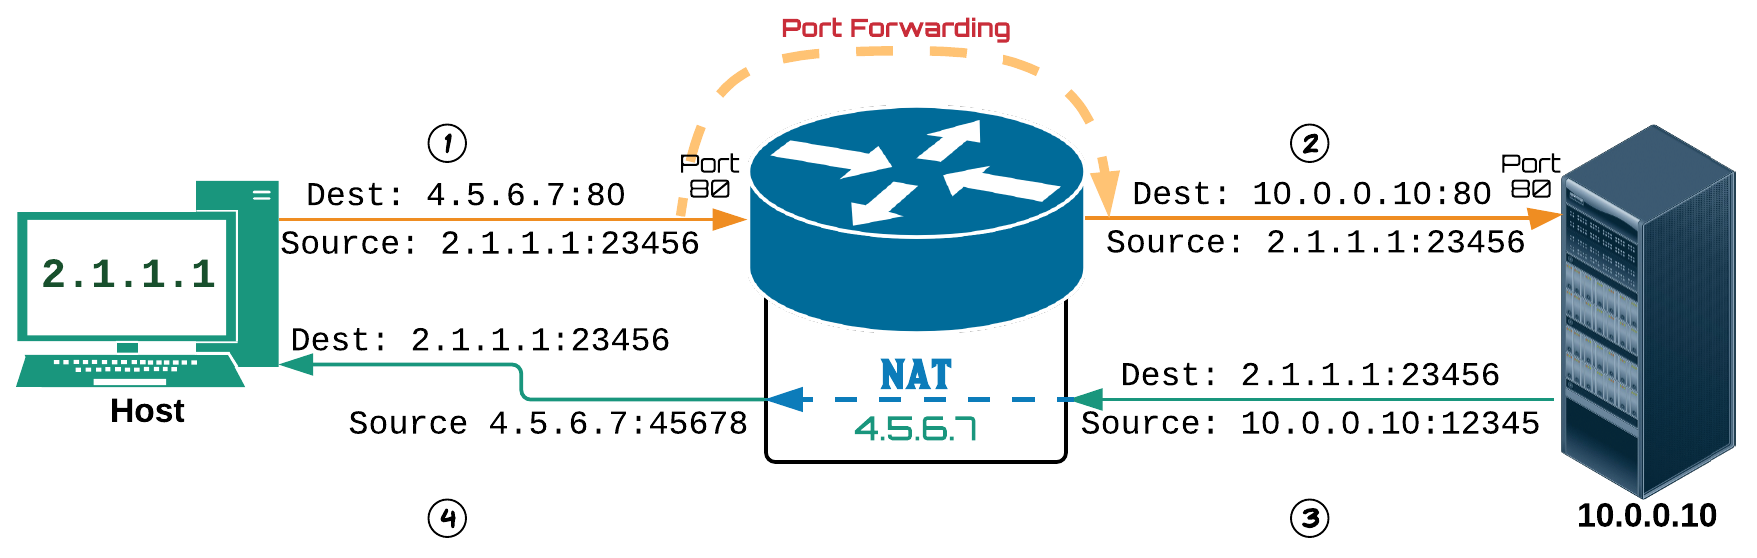
\includegraphics[width=\linewidth]{Mod2/chapters/2.7.a}
	\caption{Port Forwarding and Network Address Translation (NAT)}
	\label{fig:2}
\end{figure}

Thus, when the IP packet originates from the host it has a source IP of \verb|2.1.1.1:23456| (assuming an application uses the port 23456 to send the request). The destination IP is set to the public IP \verb|4.5.6.7:80|, which is port 80 on the router. According to the port forwarding rules, the packet is sent to the web-server at \verb|10.0.0.10:80|, where the web-server handles the request. 

Next, the response is sent from the web-server to the host. However, since the web-server has the private IP of \verb|10.0.0.10:12345| (port number is a random one based upon the application generating the request), the packet can't be allowed on the internet with a RFC 1918 address, since IP dictates that every node on the internet must have a unique public IP address. Thus, enroute to the host at \verb|2.1.1.1|, the router has to translate the private IP to a public IP (\verb|4.5.6.7|). This is called NAT. 

So, after NATting has been performed by the router, when the reply finally reaches the host, the header of the IP packet contains a source address of \verb|4.5.6.7:45678| (The port number is now a random one decided upon by the NAT device/mechanism in the router) and a destination address of \verb|2.1.1.1:23456|. In Port forwarding the Destination address (of the web-server) is changed (and not the source, since otherwise the web-server won't know who to reply to!) while in NAT, the source address (again, of the web-server) is changed. 

	\section{Configuring NAT}
Another name for the operation in which the router changes the IP address of the host on the private network to it's own public IP address is called \textbf{masquerading}. To configure NAT using this method is very easy:

\vspace{-15pt}
\begin{minted}{console}
# firewall-cmd --permanent --add-masquerade 
success
# firewall-cmd --reload
success
# firewall-cmd --list-all
public (active)
  target: default
  icmp-block-inversion: no
  interfaces: ens33 ens37 br0 team0
  sources: 10.0.0.0/24
  services: ssh dhcpv6-client
  ports: 53/tcp
  protocols: 
  masquerade: yes
  forward-ports: 
  source-ports: 
  icmp-blocks: 
  rich rules: 
\end{minted}
\vspace{-10pt}	

\noindent
Now, the hosts on the internet will only see the public IP of the router for packets that originate behind the router on the private network. 

\section{Configuring Port Forwarding}
Similar to the command to implement NATting, the command for port forwarding is also of a single line, but a bit complex. It is:

\vspace{-15pt}
\begin{minted}{console}
# firewall-cmd --permanent --add-forward-port=port=888:proto=tcp:toport=80:toaddr=10.0.99.12
success
# firewall-cmd --reload
success
# firewall-cmd --list-all
public (active)
  target: default
  icmp-block-inversion: no
  interfaces: ens33 ens37 br0 team0
  sources: 10.0.0.0/24
  services: ssh dhcpv6-client
  ports: 53/tcp
  protocols: 
  masquerade: yes
  forward-ports: port=888:proto=tcp:toport=80:toaddr=10.0.0.10
  source-ports: 
  icmp-blocks: 
  rich rules: 
\end{minted}
\vspace{-10pt}	

\noindent
In this command, the \textbf{port} of \verb|888| is the port on the router that's going to be listening for incoming connections from the internet. On receiving packets sent via \textit{proto} (protocol) of TCP on port \verb|888|, it'll forward the packet to the value specified in \textit{toport} \verb|80| on the \textit{toaddr} \verb|10.0.0.10| address. 